\documentclass[t,usenames,dvipsnames]{beamer}
\usetheme{Copenhagen}
\setbeamertemplate{headline}{} % remove toc from headers
\beamertemplatenavigationsymbolsempty

\usepackage{amsmath, tikz, xcolor}
\usetikzlibrary{arrows.meta, calc}

\title{Polar Coordinates}
\author{}
\date{}

\AtBeginSection[]
{
  \begin{frame}
    \frametitle{Objectives}
    \tableofcontents[currentsection]
  \end{frame}
}

\begin{document}

\begin{frame}
    \titlepage
\end{frame}

\section{Plot polar coordinates.}

\begin{frame}{Polar Coordinates}
    \begin{tabular}{p{0.4\textwidth}p{0.4\textwidth}}
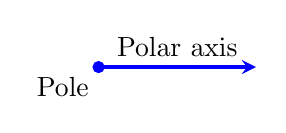
\begin{tikzpicture}
    \coordinate (O) at (0,0);
    \draw [->, >=stealth, color=blue, line width = 1.25] (O) -- (2,0) node [above, midway, black] {Polar axis}; 
    \draw [fill=blue, color=blue] (O) circle (2pt) node [below left, black] {Pole};
\end{tikzpicture}
&
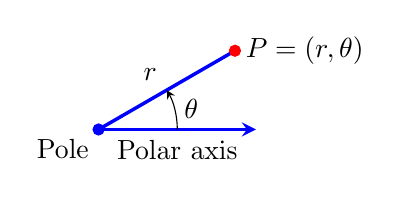
\begin{tikzpicture}
    \coordinate (O) at (0,0);
    \draw [->, >=stealth, color=blue, line width = 1.25] (O) -- (2,0) node [below, midway, black] {Polar axis}; 
    \draw [fill=blue, color=blue] (O) circle (2pt) node [below left, black] {Pole};
    \draw [-, >=stealth, color=blue, line width = 1.25] (O) -- (30:2) node [right, black] {$P=(r,\theta)$};
    \draw [color=red, fill=red] (30:2) circle (2pt);
    \draw [->,>=stealth] (0:1) arc (0:30:1) node [midway, right] {$\theta$};
    \node at (30:1) [above left] {$r$};
\end{tikzpicture}
\end{tabular}
\\[10pt]
\pause
For polar coordinates:  \newline\\
\begin{itemize}
    \item Start at the origin (pole)    \pause
    \item Go out $r$ units right ($r > 0$) or left ($r < 0$)    \pause
    \item Rotate by the amount given (\textbf{**direction**})   \pause
\end{itemize}
\vspace{10pt}

The polar coordinates of a point are $(r, \theta)$.
\end{frame}

\begin{frame}{Example 1. Plot each of the following}
\begin{minipage}{0.56\textwidth}
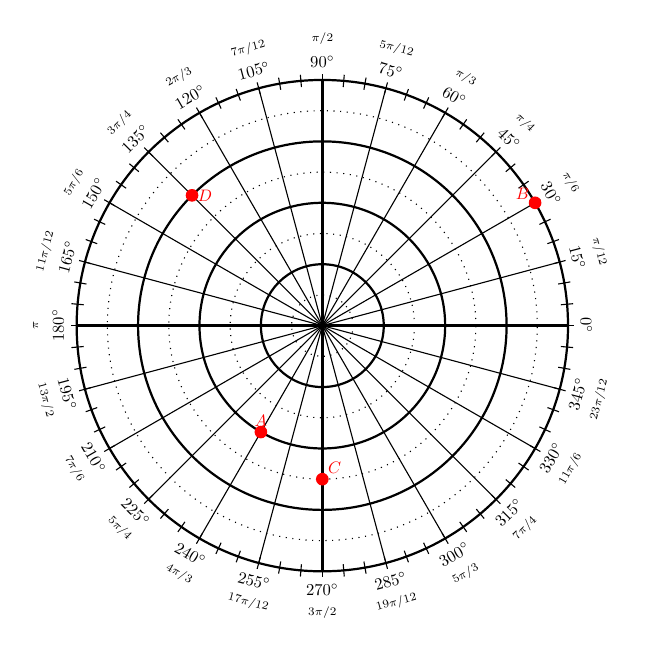
\begin{tikzpicture}[scale = 0.52, every node/.style={scale=0.6}]
    % Origin Point
    \coordinate (O) (0,0);
    % Circles
    \foreach \r in {1.5,3,...,6}
    {
        \draw[thick] (O) circle (\r cm);
    }
    
    % \foreach \r in {1.5,3,...7.5}
    % {
    %     \node at (\r, 0) [anchor=north] {\r/};
    % }
    
    \foreach \r in {0.75, 2.25,...,5.25}
    {
        \draw[dotted] (O) circle (\r cm);
    }
    
    % \node at (1.5, 0) [anchor = north west] {1};
    % \node at (3, 0) [anchor = north west] {2};
    % \node at (4.5, 0) [anchor = north west] {3};
    % \node at (6, 0) [anchor = north west] {4};
    % \node at (7.5,0) [anchor = north west] {5};
    % \foreach \r in {1.5,3,...,9}
    % {
    %     \node at (\r, 0) {\r/1.5};
    % }
    % Radial Lines
    \foreach \l in {0,15,...,360}
    {
        \draw (O) -- ++(\l:6cm);
    }
    % Thicker Radial Lines at 90 degree increments
    \foreach \l in {0,90,...,360}
    {
        \draw[very thick] (O) -- ++(\l:6cm);
    }
    % Minor Tick marks on outer circle
    \foreach \t in {0,5,...,360}
    {
        \draw (O) ++ (\t:5.85cm) -- ++(\t:0.3cm);
    }
    % Now for the fun part, the text
    % Degrees
    \node[draw=none, rotate= -90 ] at ( 0 :6.45cm) {$ 0 ^\circ$};
    \node[draw=none, rotate= -75 ] at ( 15 :6.45cm) {$ 15 ^\circ$};
    \node[draw=none, rotate= -60 ] at ( 30 :6.45cm) {$ 30 ^\circ$};
    \node[draw=none, rotate= -45 ] at ( 45 :6.45cm) {$ 45 ^\circ$};
    \node[draw=none, rotate= -30 ] at ( 60 :6.45cm) {$ 60 ^\circ$};
    \node[draw=none, rotate= -15 ] at ( 75 :6.45cm) {$ 75 ^\circ$};
    \node[draw=none, rotate= 0 ] at ( 90 :6.45cm) {$ 90 ^\circ$};
    \node[draw=none, rotate= 15 ] at ( 105 :6.45cm) {$ 105 ^\circ$};
    \node[draw=none, rotate= 30 ] at ( 120 :6.45cm) {$ 120 ^\circ$};
    \node[draw=none, rotate= 45 ] at ( 135 :6.45cm) {$ 135 ^\circ$};
    \node[draw=none, rotate= 60 ] at ( 150 :6.45cm) {$ 150 ^\circ$};
    \node[draw=none, rotate= 75 ] at ( 165 :6.45cm) {$ 165 ^\circ$};
    \node[draw=none, rotate= 90 ] at ( 180 :6.45cm) {$ 180 ^\circ$};
    \node[draw=none, rotate= 285 ] at ( 195 :6.45cm) {$ 195 ^\circ$};
    \node[draw=none, rotate= 300 ] at ( 210 :6.45cm) {$ 210 ^\circ$};
    \node[draw=none, rotate= 315 ] at ( 225 :6.45cm) {$ 225 ^\circ$};
    \node[draw=none, rotate= 330 ] at ( 240 :6.45cm) {$ 240 ^\circ$};
    \node[draw=none, rotate= 345 ] at ( 255 :6.45cm) {$ 255 ^\circ$};
    \node[draw=none, rotate= 360 ] at ( 270 :6.45cm) {$ 270 ^\circ$};
    \node[draw=none, rotate= 375 ] at ( 285 :6.45cm) {$ 285 ^\circ$};
    \node[draw=none, rotate= 390 ] at ( 300 :6.45cm) {$ 300 ^\circ$};
    \node[draw=none, rotate= 405 ] at ( 315 :6.45cm) {$ 315 ^\circ$};
    \node[draw=none, rotate= 420 ] at ( 330 :6.45cm) {$ 330 ^\circ$};
    \node[draw=none, rotate= 435 ] at ( 345 :6.45cm) {$ 345 ^\circ$};
    % Radians

    \node[draw=none, rotate= -90 ] at ( 0 :7cm) {$  $};
    \node[draw=none, rotate= -75 ] at ( 15 :7cm) {\scriptsize$ \pi/12 $};
    \node[draw=none, rotate= -60 ] at ( 30 :7cm) {\scriptsize$ \pi/6 $};
    \node[draw=none, rotate= -45 ] at ( 45 :7cm) {\scriptsize$ \pi/4 $};
    \node[draw=none, rotate= -30 ] at ( 60 :7cm) {\scriptsize$ \pi/3 $};
    \node[draw=none, rotate= -15 ] at ( 75 :7cm) {\scriptsize$ 5\pi/12 $};
    \node[draw=none, rotate= 0 ] at ( 90 :7cm) {\scriptsize$ \pi/2 $};
    \node[draw=none, rotate= 15 ] at ( 105 :7cm) {\scriptsize$ 7\pi/12 $};
    \node[draw=none, rotate= 30 ] at ( 120 :7cm) {\scriptsize$ 2\pi/3 $};
    \node[draw=none, rotate= 45 ] at ( 135 :7cm) {\scriptsize$ 3\pi/4 $};
    \node[draw=none, rotate= 60 ] at ( 150 :7cm) {\scriptsize$ 5\pi/6 $};
    \node[draw=none, rotate= 75 ] at ( 165 :7cm) {\scriptsize$ 11\pi/12 $};
    \node[draw=none, rotate= 90 ] at ( 180 :7cm) {\scriptsize$ \pi $};
    \node[draw=none, rotate= 285 ] at ( 195 :7cm) {\scriptsize$ 13\pi/2 $};
    \node[draw=none, rotate= 300 ] at ( 210 :7cm) {\scriptsize$ 7\pi/6 $};
    \node[draw=none, rotate= 315 ] at ( 225 :7cm) {\scriptsize$ 5\pi/4 $};
    \node[draw=none, rotate= 330 ] at ( 240 :7cm) {\scriptsize$ 4\pi/3 $};
    \node[draw=none, rotate= 345 ] at ( 255 :7cm) {\scriptsize$ 17\pi/12 $};
    \node[draw=none, rotate= 360 ] at ( 270 :7cm) {\scriptsize$ 3\pi/2 $};
    \node[draw=none, rotate= 375 ] at ( 285 :7cm) {\scriptsize$ 19\pi/12 $};
    \node[draw=none, rotate= 390 ] at ( 300 :7cm) {\scriptsize$ 5\pi/3 $};
    \node[draw=none, rotate= 405 ] at ( 315 :7cm) {\scriptsize$ 7\pi/4 $};
    \node[draw=none, rotate= 420 ] at ( 330 :7cm) {\scriptsize$ 11\pi/6 $};
    \node[draw=none, rotate= 435 ] at ( 345 :7cm) {\scriptsize$ 23\pi/12 $};
    
    \onslide<2->{\draw [color=red,fill=red] (240:3) circle (4pt) node [above] {$A$};}
    \onslide<4->{\draw [color=red,fill=red] (30:6) circle (4pt) node [left, yshift=0.2cm] {$B$};}
    \onslide<6->{\draw[color=red,fill=red] (270:3.75) circle (4pt) node [above right] {$C$};}
    \onslide<8->{\draw[color=red,fill=red] (135:4.5) circle (4pt) node [right] {$D$};}
\end{tikzpicture} 
\end{minipage}
\hspace{1.17cm}
\begin{minipage}{0.12\textwidth}
% (a) $A\left(2, 240^\circ\right)$ \\[15pt]
% \onslide<3->{(b) $B\left(-4,\dfrac{7\pi}{6}\right)$} \\[15pt]
% \onslide<5->{(c) $C\left(2.5,-\dfrac{5\pi}{2}\right)$} \\[15pt]
% \onslide<7->{(d) $D\left(-3, -\dfrac{\pi}{4}\right)$} \\
\begin{align*}
    &(a)\quad A\left(2, 240^\circ\right) \\[15pt]
    \onslide<3->{&(b)\quad B\left(-4,\dfrac{7\pi}{6}\right)} \\[15pt]
    \onslide<5->{&(c)\quad C\left(2.5,-\dfrac{5\pi}{2}\right)}    \\[15pt]
    \onslide<7->{&(d)\quad D\left(-3, -\dfrac{\pi}{4}\right)}
\end{align*}
\end{minipage}
\end{frame}


\section{Convert from polar to rectangular coordinates.}

\begin{frame}{Polar to Rectangular Coordinates}

\begin{center}
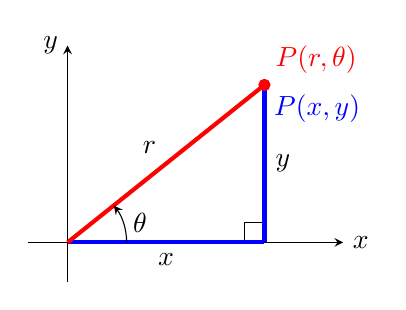
\begin{tikzpicture}
    \draw [->, >=stealth] (-0.5,0) -- (3.5,0) node [right] {$x$};
    \draw [->, >=stealth] (0,-0.5) -- (0,2.5) node [left] {$y$};
    \draw (2.5,0) rectangle +(-0.25,0.25);
    \draw [color=blue, line width = 1.5] (0,0) -- (2.5,0) node [midway, below, black] {$x$};
    \draw [color=blue, line width=1.5] (2.5,0) -- (2.5,2) node [midway, right, black] {$y$};
    \draw [color=red, line width=1.5] (0,0) -- (2.5,2) node [above right] {$P(r,\theta)$};
    \draw [color=red, fill=red] (2.5,2) circle (2pt);
    \node at (2.5,2) [below right, blue] {$P(x, y)$};
    \node at (1.25, 1) [above left] {$r$};
    \draw [->, >=stealth] (0:0.75) arc (0:38.5:0.75) node [midway, right] {$\theta$};
\end{tikzpicture}
\end{center}
\pause

\begin{align*}
    \onslide<2->{\cos\theta = \frac{x}{r} \qquad & \qquad \sin\theta = \frac{y}{r}} \\[11pt]
    \onslide<3->{x = r\cos \theta \qquad & \qquad y = r\sin \theta}   \\
\end{align*}
\end{frame}

\begin{frame}{Example 2}
Convert each to rectangular coordinates.    \newline\\
(a) \quad $\left(2, 240^\circ\right)$
\begin{align*}
    \onslide<2->{x=2\cos240^\circ \quad & \quad y = 2\sin240^\circ} \\[10pt]
    \onslide<3->{x=2\left(-\frac{1}{2}\right) \quad & \quad y = 2\left(-\frac{\sqrt{3}}{2}\right)} \\[10pt]
    \onslide<4->{x=-1 \quad & y = -\sqrt{3}} 
\end{align*}
\onslide<5->{\[(-1,\, -\sqrt{3})\]}
\end{frame}

\begin{frame}{Example 2}
    \begin{center}
    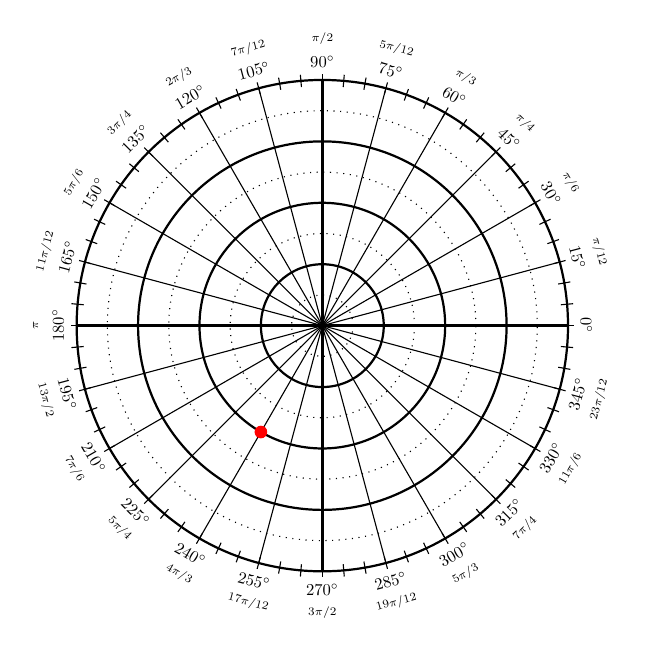
\begin{tikzpicture}[scale = 0.52, every node/.style={scale=0.6}]
    % Origin Point
    \coordinate (O) (0,0);
    % Circles
    \foreach \r in {1.5,3,...,6}
    {
        \draw[thick] (O) circle (\r cm);
    }
    
    % \foreach \r in {1.5,3,...7.5}
    % {
    %     \node at (\r, 0) [anchor=north] {\r/};
    % }
    
    \foreach \r in {0.75, 2.25,...,5.25}
    {
        \draw[dotted] (O) circle (\r cm);
    }
    
    % \node at (1.5, 0) [anchor = north west] {1};
    % \node at (3, 0) [anchor = north west] {2};
    % \node at (4.5, 0) [anchor = north west] {3};
    % \node at (6, 0) [anchor = north west] {4};
    % \node at (7.5,0) [anchor = north west] {5};
    % \foreach \r in {1.5,3,...,9}
    % {
    %     \node at (\r, 0) {\r/1.5};
    % }
    % Radial Lines
    \foreach \l in {0,15,...,360}
    {
        \draw (O) -- ++(\l:6cm);
    }
    % Thicker Radial Lines at 90 degree increments
    \foreach \l in {0,90,...,360}
    {
        \draw[very thick] (O) -- ++(\l:6cm);
    }
    % Minor Tick marks on outer circle
    \foreach \t in {0,5,...,360}
    {
        \draw (O) ++ (\t:5.85cm) -- ++(\t:0.3cm);
    }
    % Now for the fun part, the text
    % Degrees
    \node[draw=none, rotate= -90 ] at ( 0 :6.45cm) {$ 0 ^\circ$};
    \node[draw=none, rotate= -75 ] at ( 15 :6.45cm) {$ 15 ^\circ$};
    \node[draw=none, rotate= -60 ] at ( 30 :6.45cm) {$ 30 ^\circ$};
    \node[draw=none, rotate= -45 ] at ( 45 :6.45cm) {$ 45 ^\circ$};
    \node[draw=none, rotate= -30 ] at ( 60 :6.45cm) {$ 60 ^\circ$};
    \node[draw=none, rotate= -15 ] at ( 75 :6.45cm) {$ 75 ^\circ$};
    \node[draw=none, rotate= 0 ] at ( 90 :6.45cm) {$ 90 ^\circ$};
    \node[draw=none, rotate= 15 ] at ( 105 :6.45cm) {$ 105 ^\circ$};
    \node[draw=none, rotate= 30 ] at ( 120 :6.45cm) {$ 120 ^\circ$};
    \node[draw=none, rotate= 45 ] at ( 135 :6.45cm) {$ 135 ^\circ$};
    \node[draw=none, rotate= 60 ] at ( 150 :6.45cm) {$ 150 ^\circ$};
    \node[draw=none, rotate= 75 ] at ( 165 :6.45cm) {$ 165 ^\circ$};
    \node[draw=none, rotate= 90 ] at ( 180 :6.45cm) {$ 180 ^\circ$};
    \node[draw=none, rotate= 285 ] at ( 195 :6.45cm) {$ 195 ^\circ$};
    \node[draw=none, rotate= 300 ] at ( 210 :6.45cm) {$ 210 ^\circ$};
    \node[draw=none, rotate= 315 ] at ( 225 :6.45cm) {$ 225 ^\circ$};
    \node[draw=none, rotate= 330 ] at ( 240 :6.45cm) {$ 240 ^\circ$};
    \node[draw=none, rotate= 345 ] at ( 255 :6.45cm) {$ 255 ^\circ$};
    \node[draw=none, rotate= 360 ] at ( 270 :6.45cm) {$ 270 ^\circ$};
    \node[draw=none, rotate= 375 ] at ( 285 :6.45cm) {$ 285 ^\circ$};
    \node[draw=none, rotate= 390 ] at ( 300 :6.45cm) {$ 300 ^\circ$};
    \node[draw=none, rotate= 405 ] at ( 315 :6.45cm) {$ 315 ^\circ$};
    \node[draw=none, rotate= 420 ] at ( 330 :6.45cm) {$ 330 ^\circ$};
    \node[draw=none, rotate= 435 ] at ( 345 :6.45cm) {$ 345 ^\circ$};
    % Radians

    \node[draw=none, rotate= -90 ] at ( 0 :7cm) {$  $};
    \node[draw=none, rotate= -75 ] at ( 15 :7cm) {\scriptsize$ \pi/12 $};
    \node[draw=none, rotate= -60 ] at ( 30 :7cm) {\scriptsize$ \pi/6 $};
    \node[draw=none, rotate= -45 ] at ( 45 :7cm) {\scriptsize$ \pi/4 $};
    \node[draw=none, rotate= -30 ] at ( 60 :7cm) {\scriptsize$ \pi/3 $};
    \node[draw=none, rotate= -15 ] at ( 75 :7cm) {\scriptsize$ 5\pi/12 $};
    \node[draw=none, rotate= 0 ] at ( 90 :7cm) {\scriptsize$ \pi/2 $};
    \node[draw=none, rotate= 15 ] at ( 105 :7cm) {\scriptsize$ 7\pi/12 $};
    \node[draw=none, rotate= 30 ] at ( 120 :7cm) {\scriptsize$ 2\pi/3 $};
    \node[draw=none, rotate= 45 ] at ( 135 :7cm) {\scriptsize$ 3\pi/4 $};
    \node[draw=none, rotate= 60 ] at ( 150 :7cm) {\scriptsize$ 5\pi/6 $};
    \node[draw=none, rotate= 75 ] at ( 165 :7cm) {\scriptsize$ 11\pi/12 $};
    \node[draw=none, rotate= 90 ] at ( 180 :7cm) {\scriptsize$ \pi $};
    \node[draw=none, rotate= 285 ] at ( 195 :7cm) {\scriptsize$ 13\pi/2 $};
    \node[draw=none, rotate= 300 ] at ( 210 :7cm) {\scriptsize$ 7\pi/6 $};
    \node[draw=none, rotate= 315 ] at ( 225 :7cm) {\scriptsize$ 5\pi/4 $};
    \node[draw=none, rotate= 330 ] at ( 240 :7cm) {\scriptsize$ 4\pi/3 $};
    \node[draw=none, rotate= 345 ] at ( 255 :7cm) {\scriptsize$ 17\pi/12 $};
    \node[draw=none, rotate= 360 ] at ( 270 :7cm) {\scriptsize$ 3\pi/2 $};
    \node[draw=none, rotate= 375 ] at ( 285 :7cm) {\scriptsize$ 19\pi/12 $};
    \node[draw=none, rotate= 390 ] at ( 300 :7cm) {\scriptsize$ 5\pi/3 $};
    \node[draw=none, rotate= 405 ] at ( 315 :7cm) {\scriptsize$ 7\pi/4 $};
    \node[draw=none, rotate= 420 ] at ( 330 :7cm) {\scriptsize$ 11\pi/6 $};
    \node[draw=none, rotate= 435 ] at ( 345 :7cm) {\scriptsize$ 23\pi/12 $};
    \draw [color=red,fill=red] (240:3) circle (4pt);
    \end{tikzpicture}
    \end{center}
\end{frame}

\begin{frame}{Example 2}
\begin{center}
\begin{tikzpicture}[scale=0.52]
    \draw [<->,>=stealth,very thick] (-6,0) -- (6,0) node [right] {$x$};
    \draw [<->,>=stealth,very thick] (0,-6) -- (0,6) node [right] {$y$};
    \foreach \x in {-4.5,-3,...,4.5}
    \draw [thick] (\x,0.2) -- (\x,-0.2);
    \foreach \y in {-4.5,-3,...,4.5}
    \draw [thick] (0.2,\y) -- (-0.2,\y);
    \draw [color=red,fill=red] (240:3) circle (4pt);
\end{tikzpicture}
\end{center}
\end{frame}

\begin{frame}{Example 2}
(b) \quad $\left(-4, \dfrac{7\pi}{6}\right)$
\begin{align*}
    \onslide<2->{x = -4\cos\left(\frac{7\pi}{6}\right) \quad & \quad y = -4\sin\left(\frac{7\pi}{6}\right)} \\[10pt]
    \onslide<3->{x = -4\left(-\frac{\sqrt{3}}{2}\right) \quad & \quad y = -4\left(-\frac{1}{2}\right)} \\[10pt]
    \onslide<4->{x = 2\sqrt{3} \quad & \quad y = 2}
\end{align*}
\onslide<5->{\[\left(2\sqrt{3}, \, 2\right) \]}
\end{frame}

\begin{frame}{Example 2}
(c) \quad $\left(2.5, -\dfrac{5\pi}{2}\right)$
\begin{align*}
    \onslide<2->{x = 2.5\cos\left(-\frac{5\pi}{2}\right) \quad & \quad y = 2.5\sin\left(-\frac{5\pi}{2}\right)} \\[10pt]
    \onslide<3->{x = 2.5\left(0\right) \quad & \quad y = 2.5\left(-1\right)} \\[10pt]
    \onslide<4->{x = 0 \quad & \quad y = -2.5}
\end{align*}
\onslide<5->{\[\left(0, \, -2.5\right) \]}
\end{frame}

\begin{frame}{Example 2}
(d) \quad $\left(-3, -\dfrac{\pi}{4}\right)$
\begin{align*}
    \onslide<2->{x = -3\cos\left(-\frac{\pi}{4}\right) \quad & \quad y = -3\sin\left(-\frac{\pi}{4}\right)} \\[10pt]
    \onslide<3->{x = -3\left(\frac{\sqrt{2}}{2}\right) \quad & \quad y = -3\left(-\frac{\sqrt{2}}{2}\right)} \\[10pt]
    \onslide<4->{x = -\frac{3\sqrt{2}}{2} \quad & \quad y = \frac{3\sqrt{2}}{2}}
\end{align*}
\onslide<5->{\[\left(-\frac{3\sqrt{2}}{2}, \, \frac{3\sqrt{2}}{2}\right) \]}
\end{frame}

\section{Convert from rectangular to polar coordinates.}

\begin{frame}{Rectangular to Polar}
\begin{center}
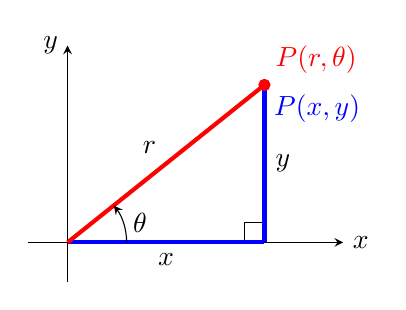
\begin{tikzpicture}
    \draw [->, >=stealth] (-0.5,0) -- (3.5,0) node [right] {$x$};
    \draw [->, >=stealth] (0,-0.5) -- (0,2.5) node [left] {$y$};
    \draw (2.5,0) rectangle +(-0.25,0.25);
    \draw [color=blue, line width = 1.5] (0,0) -- (2.5,0) node [midway, below, black] {$x$};
    \draw [color=blue, line width=1.5] (2.5,0) -- (2.5,2) node [midway, right, black] {$y$};
    \draw [color=red, line width=1.5] (0,0) -- (2.5,2) node [above right] {$P(r,\theta)$};
    \draw [color=red, fill=red] (2.5,2) circle (2pt);
    \node at (2.5,2) [below right, blue] {$P(x, y)$};
    \node at (1.25, 1) [above left] {$r$};
    \draw [->, >=stealth] (0:0.75) arc (0:38.5:0.75) node [midway, right] {$\theta$};
\end{tikzpicture}
\end{center}
\pause
\[
r = \sqrt{x^2+y^2} \qquad \onslide<3->{\theta' = \tan^{-1}\left| \frac{y}{x} \right|}
\]
\vspace{15pt}
\onslide<4->{where $\theta '$ is the \underline{reference angle} used to find the total angle rotated, $\theta$.}
\end{frame}

\begin{frame}{Example 3}
Convert each of the following to polar coordinates. \newline\\
(a) \quad $\left(2, -2\sqrt{3}\right)$   \newline\\
\begin{minipage}{0.5\textwidth}
\begin{tikzpicture}[scale=0.9]
\draw[<->,>=stealth] (-2.5,0) -- (2.5,0) node [right] {$x$};
\draw[<->,>=stealth] (0,-2.5) -- (0,2.5) node [above] {$y$};
\coordinate (A) at (1,-1.7);
\draw[fill=black] (A) circle (2pt);
\onslide<2->{\draw (0,0) -- (A) -- node [right] {\scriptsize $-2\sqrt{3}$} (1,0) -- node [above] {\scriptsize $2$} cycle;}
\onslide<4->{\node at (0.3,-0.15) {\scriptsize $\theta'$};}
\onslide<4->{\node at (300:1) [left] {\scriptsize 4};}
\onslide<6->{\node at (0.3,-0.15) [color=white,fill=white] {};}
\onslide<6->{\node at (0.35,-0.15) {\scriptsize $60^\circ$};}
\onslide<7->{\draw[->,>=stealth,color=red] (0.75,0) arc (0:300:0.75) node [xshift=-1cm, yshift=1.25cm] {\scriptsize $300^\circ$};}
\end{tikzpicture}
\end{minipage}
\hspace{-0.5cm}
\begin{minipage}{0.5\textwidth}
\begin{align*}
    \onslide<3->{r &= \sqrt{2^2 + (2\sqrt{3})^2} = \sqrt{16} = 4}  \\[8pt]
    \onslide<5->{\theta' &= \tan^{-1}\left|\frac{-2\sqrt{3}}{2}\right| = 60^\circ}    \\[8pt]
    \onslide<7->{\theta &= 300^\circ} \\[8pt]
    & \onslide<8->{\left(4, \frac{5\pi}{3}\right)} \\
\end{align*}
\end{minipage}
\end{frame}

\begin{frame}{Example 3}
(b) \quad $(-3, -3)$ \newline\\
\begin{minipage}{0.4\textwidth}
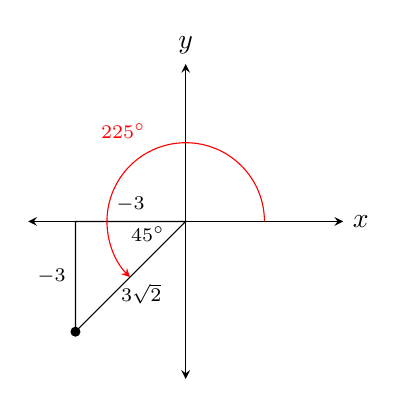
\begin{tikzpicture}[scale=0.8]
\draw[<->,>=stealth] (-2.5,0) -- (2.5,0) node [right] {$x$};
\draw[<->,>=stealth] (0,-2.5) -- (0,2.5) node [above] {$y$};
\coordinate (A) at (-1.75,-1.75);
\draw [fill=black] (A) circle (2pt);
\onslide<2->{\draw (0,0) -- (A) -- node [left] {\scriptsize $-3$} (-1.75,0) -- node [above] {\scriptsize $-3$} cycle;}
\onslide<4->{\node at (-0.5,-0.2) {\scriptsize $\theta'$};}
\onslide<4->{\node at (225:1) [below, yshift=-0.1cm] {\scriptsize $3\sqrt{2}$};}
\onslide<6->{\node at (-0.5,-0.2) [color=white,fill=white] {};}
\onslide<6->{\node at (-0.6,-0.2) {\scriptsize $45^\circ$};}
\onslide<7->{\draw[->,>=stealth,color=red] (1.25,0) arc (0:225:1.25) node [midway, above left] {\scriptsize $225^\circ$};}
\end{tikzpicture}
\end{minipage}
\hspace{0.5cm}
\begin{minipage}{0.5\textwidth}
\begin{align*}
    \onslide<3->{r &= \sqrt{3^2 + 3^2} = 3\sqrt{2}}  \\[8pt]
    \onslide<5->{\theta' &= \tan^{-1}\left|\frac{-3}{-3}\right| = 45^\circ}    \\[8pt]
    \onslide<7->{\theta &= 225^\circ} \\[8pt]
    & \onslide<8->{\left(3\sqrt{2}, \frac{5\pi}{4}\right)} \\
\end{align*}
\end{minipage}
\end{frame}


\begin{frame}{Example 3}
(c) \quad $(0, -3)$ \newline\\
\begin{minipage}{0.4\textwidth}
\begin{tikzpicture}[scale=0.8]
\draw[<->,>=stealth] (-2.5,0) -- (2.5,0) node [right] {$x$};
\draw[<->,>=stealth] (0,-2.5) -- (0,2.5) node [above] {$y$};
\draw (-0.15,-1.75) -- (0.15,-1.75) node [right] {\scriptsize $-3$};
\coordinate (A) at (0,-1.75);
\draw [fill=black] (A) circle (2pt);
\onslide<2->{\node at (0,-0.75) [right, red] {\scriptsize $r = 3$};}
\onslide<3->{\draw[->,>=stealth,color=red] (1,0) arc (0:270:1) node [midway, above left] {\scriptsize $270^\circ$};}
\end{tikzpicture}
\end{minipage}
\hspace{0.5cm}
\begin{minipage}{0.5\textwidth}
\begin{align*}
    \onslide<2->{r &= 3}  \\[12pt]
    \onslide<4->{\theta &= \frac{3\pi}{2}} \\[12pt]
    \onslide<5->{&\left(3, \frac{3\pi}{2}\right)}
\end{align*}
\end{minipage}
\end{frame}


\begin{frame}{Example 3}
(d) \quad $(-3, 4)$ \newline\\
\begin{minipage}{0.4\textwidth}
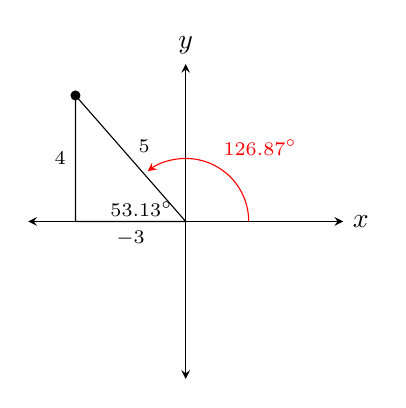
\begin{tikzpicture}[scale=0.8]
\draw[<->,>=stealth] (-2.5,0) -- (2.5,0) node [right] {$x$};
\draw[<->,>=stealth] (0,-2.5) -- (0,2.5) node [above] {$y$};
\coordinate (A) at (-1.75,2);
\draw [fill=black] (A) circle (2pt);
\onslide<2->{\draw (0,0) -- (A) -- node [left] {\scriptsize $4$} (-1.75,0) -- node [below] {\scriptsize $-3$} cycle;}
\onslide<4->{\node at (-0.5,0.2) {\scriptsize $\theta'$};}
\onslide<4->{\node at (127:1.5) [right] {\scriptsize $5$};}
\onslide<6->{\node at (-0.5,0.2) [color=white,fill=white] {};}
\onslide<6->{\node at (-0.7,0.2) {\scriptsize $53.13^\circ$};}
\onslide<7->{\draw[->,>=stealth,color=red] (1,0) arc (0:127:1) node [midway, above right] {\scriptsize $126.87^\circ$};}
\end{tikzpicture}
\end{minipage}
\hspace{0.5cm}
\begin{minipage}{0.5\textwidth}
\begin{align*}
    \onslide<3->{r &= \sqrt{3^2 + 4^2} = 5}  \\[8pt]
    \onslide<5->{\theta' &= \tan^{-1}\left|\frac{4}{-3}\right| \approx 53.13^\circ}    \\[8pt]
    \onslide<7->{\theta &\approx 126.87^\circ} \\[8pt]
    \onslide<8->{&\left(5, \pi - \tan^{-1}\left(\frac{4}{3}\right)\right)} \\
\end{align*}
\end{minipage}
\end{frame}


\section{Convert rectangular equations to polar equations.}

\begin{frame}{Rectangular and Polar Equations}
We can use the relationship between rectangular and polar coordinates to convert equations of one form to the other.  \newline\\  \pause

\begin{tabular}{p{0.4\textwidth}p{0.4\textwidth}}
    \onslide<2->{$x = r\cos \theta$}  & \onslide<3->{$x^2 + y^2 = r^2$}  \\
    \onslide<2->{$y = r\sin\theta$}   & \onslide<3->{$\tan\theta = \dfrac{y}{x}$}  \\ 
\end{tabular}
\end{frame}

\begin{frame}{Example 4}
    Convert each to polar equations.    \newline\\
(a) \quad $y=-x$ 
\begin{align*}
    \onslide<2->{{\color{red}y}&=-{\color{blue}x}} \\[8pt]
    \onslide<3->{{\color{red}r\sin\theta} &= - {\color{blue}r\cos\theta}} \\[8pt]
    \onslide<4->{r\cos\theta\ + r\sin\theta &= 0} \\[8pt]
    \onslide<5->{r(\cos\theta + \sin\theta) &= 0}
\end{align*}
\end{frame}

\begin{frame}{Example 4}
\[r(\cos\theta + \sin\theta) = 0\]
\begin{align*}
    \onslide<2->{r &= 0 & \cos\theta + \sin\theta &= 0} \\[8pt]
    \onslide<3->{&& \cos\theta &= -\sin\theta} \\[8pt]
    \onslide<4->{&&{\color{red}\theta} &= {\color{red}-\frac{\pi}{4}}}
\end{align*}
\end{frame}

\begin{frame}{Example 4}
(b) \quad $y=x^2$
\begin{align*}
    \onslide<2->{{\color{red}r\sin\theta} &= \left({\color{blue}r\cos\theta}\right)^2} \\[8pt]
    \onslide<3->{r\sin\theta &= r^2\cos^2\theta} \\[8pt]
    \onslide<4->{r\sin\theta - r^2\cos^2\theta &= 0} \\[8pt]
    \onslide<5->{r\left(\sin\theta - r\cos^2\theta\right) &= 0} 
\end{align*}
\begin{align*}
    \onslide<6->{r &= 0 & \sin\theta - r\cos^2\theta &= 0} 
\end{align*}
\end{frame}

\begin{frame}{Example 4}
\[ \sin\theta - r\cos^2\theta = 0\]
\begin{align*}
    \onslide<2->{\sin\theta &= r\cos^2\theta} \\[8pt]
    \onslide<3->{r &= \frac{\sin\theta}{\cos^2\theta}} \\[10pt]
    \onslide<4->{r &= \left(\frac{\sin\theta}{\cos\theta}\right)\left(\frac{1}{\cos\theta}\right)}    \\[10pt]
    \onslide<5->{r &= \tan\theta \cdot \sec\theta}
\end{align*}
\end{frame}

\begin{frame}{Example 4}
(c) \quad $(x-3)^2 + y^2 = 9$
\begin{align*}
    \onslide<2->{(r\cos\theta - 3)^2 + (r\sin\theta)^2 &= 9} \\[6pt]
    \onslide<3->{r^2\cos^2\theta - 6r\cos\theta + 9 + r^2\sin^2\theta &= 9} \\[6pt]
    \onslide<4->{r^2\cos^2\theta + r^2\sin^2\theta - 6r\cos\theta &= 0} \\[6pt]
    \onslide<5->{r^2\left(\cos^2\theta + \sin^2\theta\right) - 6r\cos\theta &= 0} \\[6pt]
    \onslide<6->{r^2 - 6r\cos\theta &= 0} \\[6pt]
    \onslide<7->{r(r-6\cos\theta) &= 0}
\end{align*}
\begin{align*}
\onslide<8->{r &= 0 & r-6\cos\theta &= 0}
\end{align*}
\end{frame}

\begin{frame}{Example 4}
    \[r-6\cos\theta = 0\]
\onslide<2->{\[r = 6\cos\theta \]}
\end{frame}

\section{Convert polar equations to rectangular equations}


\begin{frame}{Example 5}
Convert each of the following to rectangular equations. \newline\\
(a) \quad $r = -3$
\begin{align*}
    \onslide<2->{r &= -3} \\[8pt]
    \onslide<3->{r^2 &= 9} \\[8pt]
    \onslide<4->{x^2+y^2 &= 9} 
\end{align*}
\end{frame}

\begin{frame}{Example 5}
(b) \quad $\theta = \dfrac{4\pi}{3}$
\begin{align*}
    \onslide<2->{\theta &= \frac{4\pi}{3}} \\[8pt]
    \onslide<3->{\tan \theta &= \tan\left(\frac{4\pi}{3}\right)} \\[8pt]
    \onslide<4->{\frac{y}{x} &= \sqrt{3}} \\[8pt]
    \onslide<5->{y &= x\sqrt{3}} \\
\end{align*}
\end{frame}

\begin{frame}{Example 5}
(c) \quad $r = 1 - \cos\theta$
\begin{align*}
    \onslide<2->{r &= 1 - \cos\theta} \\[6pt]
    \onslide<3->{r \cdot {\color{red}r} &= {\color{red}r}(1-\cos\theta)} \\[6pt]
    \onslide<4->{r^2 &= r-r\cos\theta} \\[6pt]
    \onslide<5->{x^2 + y^2 &= r - x} \\[6pt]
    \onslide<6->{x^2 + y^2 + x &= r} \\[6pt]
    \onslide<7->{\left(x^2 + y^2 + x\right)^2 &= x^2 + y^2}
\end{align*}
\end{frame}


\end{document}
